% ============================================================================
\section{Bayesian Networks (Car Tracking)}
\label{sec:bayesian}
% Source: assignments/06_bayesian/index.html
% ============================================================================

Set-up: our car's position $a_t$ is observed. The other car's location is $C_t$ (hidden). The microphone reading
is $D_t\sim\mathcal N(\norm{a_t-C_t}_2,\sigma^2)$. Lower-case $p(\cdot)$ denotes local conditional distributions
of the Bayesian network; upper-case $\P(\cdot)$ denotes joint or posterior quantities obtained by inference.

% ----------------------------------------------------------------------------
\subsection{Emission probabilities}
The other car is stationary: $C_t=C$ for all $t$.

\problempart{1a}{Bayesian network}
\question{Draw the Bayesian network over $C,D_1,D_2,D_3,a_1,a_2,a_3$, shading the variables observed after $t=3$.}
\expect{A legible drawing with one arrow from each parent of each variable.}
\begin{solution}
\todo{draw with TikZ: nodes use the styles latent / obs, arrows use edge}
% \begin{center}\begin{tikzpicture}[node distance=18mm]
%   \node[latent] (C) {$C$};
%   ...
% \end{tikzpicture}\end{center}
\end{solution}

\problempart{1b}{Joint distribution}
\question{Express $\P(C=c,D_1=d_1,D_2=d_2,D_3=d_3)$ using only local conditional distributions
($a_1,a_2,a_3$ are known with probability 1).}
\expect{A formula that uses only local conditional distributions.}
\begin{solution}
\todo{answer}
\end{solution}

\problempart{1c}{\texttt{ExactInference.observe}}
\codepart{6.1c}

% ----------------------------------------------------------------------------
\subsection{Transition probabilities}
The other car moves according to $p(c_{t+1}\mid c_t)$, given in code as \texttt{self.transProb}.

\problempart{2a}{Bayesian network}
\question{Draw the Bayesian network over $C_1,C_2,C_3,D_1,D_2,D_3,a_1,a_2,a_3$, shading the variables observed after $t=3$.}
\expect{A legible drawing with one arrow from each parent of each variable.}
\begin{solution}
\todo{TikZ drawing}
\end{solution}

\problempart{2b}{Joint distribution}
\question{Express $\P(C_1=c_1,C_2=c_2,C_3=c_3,D_1=d_1,D_2=d_2,D_3=d_3)$ using only local conditional distributions.}
\expect{A formula that uses only local conditional distributions.}
\begin{solution}
\todo{answer}
\end{solution}

\problempart{2c}{\texttt{ExactInference.elapseTime}}
\codepart{6.2c}

% ----------------------------------------------------------------------------
\subsection{Which car is it?}
With $K$ cars, we observe only $\mathbf E_t=[E_{t1},\dots,E_{tK}]$, a uniformly random permutation of the true
noisy distances $\mathbf D_t=[D_{t1},\dots,D_{tK}]$, so a reading cannot be attributed to a specific car. All
distances are distinct.

\begin{figure}[H]\centering
  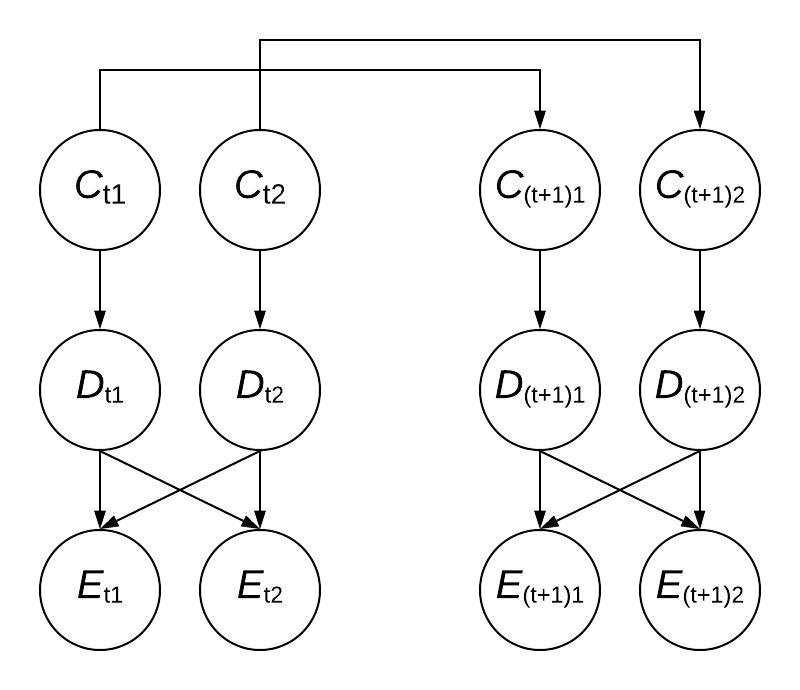
\includegraphics[width=0.45\linewidth]{06_bayesian/Q4_diag.jpeg}
  \caption{Flow of information for $K=2$ (from the handout; not a Bayesian network).}
\end{figure}

\problempart{3a}{Posterior for $K=2$, $T=1$}
\question{Write $p(C_{11}=c_{11},C_{12}=c_{12}\mid\mathbf E_1=\mathbf e_1)$ in terms of the Gaussian pdf
$p_{\mathcal N}(v;\mu,\sigma^2)$ and the priors $p(c_{11}),p(c_{12})$, without $D_{11},D_{12}$.
(For $K=1$: $p(c_{11}\mid\mathbf e_1)\propto p(c_{11})\,p_{\mathcal N}(e_{11};\norm{a_1-c_{11}}_2,\sigma^2)$.)}
\expect{The expression (proportionality is fine) and the steps taken to derive it.}
\begin{solution}
\todo{answer}
\end{solution}

\problempart{3b}{At least $K!$ maximisers}
\question{If the prior $p(c_{1i})$ is the same for every car, show that at least $K!$ assignments
$(c_{11},\dots,c_{1K})$ attain the maximum of $p(C_{11}=c_{11},\dots,C_{1K}=c_{1K}\mid\mathbf E_1=\mathbf e_1)$
(assume the maximising locations are distinct).}
\expect{A short mathematical argument or a concise explanation.}
\begin{solution}
\todo{answer}
\end{solution}

% ----------------------------------------------------------------------------
\subsection{Ethics in advanced technologies}

\problempart{4a}{Camera data misuse (dual use)}
\question{Self-driving cars often use cameras, which capture faces, licence plates and more. How might camera
data or its readings be misused, and what measures could pre-empt the misuse (or why are there none)?}
\expect{4--6 sentences.}
\begin{solution}
\todo{answer}
\end{solution}

\problempart{4b}{Sensor deception}
\codepart{6.4b}
Observed distance after the attack:
$D'_t=\frac{1}{1+\text{skewness}^2}\,D_t+\sqrt{\frac{2}{1+\text{skewness}^2}}$, implemented in
\texttt{ExactInferenceWithSensorDeception.observe}.

\problempart{4c}{Guarding against sensor deception}
\question{How could you guard against sensor deception if the type of attack is known in advance? (Hint: sensor redundancy.)}
\expect{1--2 sentences.}
\begin{solution}
\todo{answer}
\end{solution}

\problempart{4d}{Particle filtering vs.\ exact inference}
\question{Run \texttt{python drive.py -a -d -k 3 -i particleFilter}. How does the simulation differ from exact inference, and why?}
\expect{1--2 sentences.}
\begin{solution}
\todo{answer}
\end{solution}

\problempart{4e}{Privacy--accuracy trade-off}
\question{Particle filtering can run on-device (more private and secure) but is less accurate than cloud-based
exact inference. How would you weigh this trade-off?}
\expect{3--5 sentences.}
\begin{solution}
\todo{answer}
\end{solution}

\problempart{4f}{Adversarial attack on camera-based training}
\question{A camera-based autonomous vehicle is further trained on customers' anonymised camera data. Name an
adversarial attack, its potential impact on the vehicle, and a mitigation.}
\expect{3--5 sentences.}
\begin{solution}
\todo{answer}
\end{solution}
